%% abtex2-modelo-trabalho-academico.tex, v-1.9.7 laurocesar
%% Copyright 2012-2018 by abnTeX2 group at http://www.abntex.net.br/ 
%%
%% This work may be distributed and/or modified under the
%% conditions of the LaTeX Project Public License, either version 1.3
%% of this license or (at your option) any later version.
%% The latest version of this license is in
%%   http://www.latex-project.org/lppl.txt
%% and version 1.3 or later is part of all distributions of LaTeX
%% version 2005/12/01 or later.
%%
%% This work has the LPPL maintenance status `maintained'.
%% 
%% The Current Maintainer of this work is the abnTeX2 team, led
%% by Lauro César Araujo. Further information are available on 
%% http://www.abntex.net.br/
%%
%% This work consists of the files abntex2-modelo-trabalho-academico.tex,
%% abntex2-modelo-include-comandos and abntex2-modelo-references.bib
%%
% ------------------------------------------------------------------------
% ------------------------------------------------------------------------
% abnTeX2: Modelo de Trabalho Academico (tese de doutorado, dissertacao de
% mestrado e trabalhos monograficos em geral) em conformidade com 
% ABNT NBR 14724:2011: Informacao e documentacao - Trabalhos academicos -
% Apresentacao
% ------------------------------------------------------------------------
% ------------------------------------------------------------------------
%%
%% Documento ajustado para PCS-EPUSP em 15/mar/2023 por Cintia Borges Margi
%% Monografia do TCC "Livraria Digital com Oblivious Transfer" (2026).
%% Conteúdo migrado de docs/especificacao/especificacao.tex (v3).
%% Compilar: latexmk -pdf main
% ------------------------------------------------------------------------
%%
\documentclass[
	% -- opções da classe memoir --
	12pt,				% tamanho da fonte
	openright,			% capítulos começam em pág ímpar (insere página vazia caso preciso)
	twoside,			% para impressão em recto e verso. Oposto a oneside
	a4paper,			% tamanho do papel. 
	% -- opções da classe abntex2 --
	%chapter=TITLE,		% títulos de capítulos convertidos em letras maiúsculas
	%section=TITLE,		% títulos de seções convertidos em letras maiúsculas
	%subsection=TITLE,	% títulos de subseções convertidos em letras maiúsculas
	%subsubsection=TITLE,% títulos de subsubseções convertidos em letras maiúsculas
	% -- opções do pacote babel --
	english,			% idioma adicional para hifenização
	french,				% idioma adicional para hifenização
	spanish,			% idioma adicional para hifenização
	brazil				% o último idioma é o principal do documento
	]{abntex2}

% ---
% Pacotes básicos 
% ---
\usepackage{lmodern}			% Usa a fonte Latin Modern			
\usepackage[T1]{fontenc}		% Selecao de codigos de fonte.
\usepackage[utf8]{inputenc}		% Codificacao do documento (conversão automática dos acentos)
\usepackage{indentfirst}		% Indenta o primeiro parágrafo de cada seção.
\usepackage{color}				% Controle das cores
\usepackage{graphicx}			% Inclusão de gráficos
\usepackage{microtype} 			% para melhorias de justificação
% ---
		
% ---
% Pacotes adicionais deste trabalho
% ---
\usepackage{amsmath, amssymb}
\usepackage{booktabs}
\usepackage{array}
\usepackage{tabularx}
\usepackage{tikz}
\usetikzlibrary{arrows.meta}
% ---

% ---
% Pacotes de citações
% ---
\usepackage[brazilian,hyperpageref]{backref}	 % Paginas com as citações na bibl
\usepackage[alf]{abntex2cite}	% Citações padrão ABNT

%% CBM: pacote para incluir a ficha catalográfica como pdf
\usepackage[final]{pdfpages}

% --- 
% CONFIGURAÇÕES DE PACOTES
% --- 

% ---
% Configurações do pacote backref
% Usado sem a opção hyperpageref de backref
\renewcommand{\backrefpagesname}{Citado na(s) página(s):~}
% Texto padrão antes do número das páginas
\renewcommand{\backref}{}
% Define os textos da citação
\renewcommand*{\backrefalt}[4]{
	\ifcase #1 %
		Nenhuma citação no texto.%
	\or
		Citado na página #2.%
	\else
		Citado #1 vezes nas páginas #2.%
	\fi}%
% ---

% ---
% Informações de dados para CAPA e FOLHA DE ROSTO
% ---
\titulo{Aplicação de Protocolos de Oblivious Transfer para Preservação de Privacidade em Transações Digitais}
\autor{João Paulo Garcia\\João Pedro Magalhães\\Miguel Luis Schwengber}
\local{São Paulo, SP}
\data{2026}
\orientador{Prof. Dr. Thales Areco Bandiera Paiva}
\instituicao{%
  Universidade de São Paulo -- USP
  \par
  Escola Politécnica
  \par
  Departamento de Engenharia de Computação e Sistemas Digitais (PCS)}
\tipotrabalho{Monografia de Conclusão de curso (Graduação)}
% O preambulo deve conter o tipo do trabalho, o objetivo, 
% o nome da instituição e a área de concentração 
\preambulo{Trabalho de conclusão de curso apresentado ao Departamento de Engenharia de Computação e Sistemas Digitais da Escola Politécnica da Universidade de São Paulo para obtenção do Título de Engenheiro.}
% ---


% ---
% Configurações de aparência do PDF final

% alterando o aspecto da cor azul
\definecolor{blue}{RGB}{41,5,195}

% informações do PDF
\makeatletter
\hypersetup{
     	%pagebackref=true,
		pdftitle={\@title}, 
		pdfauthor={\@author},
    	pdfsubject={\imprimirpreambulo},
	    pdfcreator={LaTeX with abnTeX2},
		pdfkeywords={oblivious transfer}{privacidade}{assinatura cega}{comércio eletrônico}{criptografia}, 
		colorlinks=true,       		% false: boxed links; true: colored links
    	linkcolor=blue,          	% color of internal links
    	citecolor=blue,        		% color of links to bibliography
    	filecolor=magenta,      		% color of file links
		urlcolor=blue,
		bookmarksdepth=4
}
\makeatother
% --- 

% ---
% Posiciona figuras e tabelas no topo da página quando adicionadas sozinhas
% em um página em branco. Ver https://github.com/abntex/abntex2/issues/170
\makeatletter
\setlength{\@fptop}{5pt} % Set distance from top of page to first float
\makeatother
% ---

% ---
% Possibilita criação de Quadros e Lista de quadros.
% Ver https://github.com/abntex/abntex2/issues/176
%
\newcommand{\quadroname}{Quadro}
\newcommand{\listofquadrosname}{Lista de quadros}

\newfloat[chapter]{quadro}{loq}{\quadroname}
\newlistof{listofquadros}{loq}{\listofquadrosname}
\newlistentry{quadro}{loq}{0}

% configurações para atender às regras da ABNT
\setfloatadjustment{quadro}{\centering}
\counterwithout{quadro}{chapter}
\renewcommand{\cftquadroname}{\quadroname\space} 
\renewcommand*{\cftquadroaftersnum}{\hfill--\hfill}

\setfloatlocations{quadro}{hbtp} % Ver https://github.com/abntex/abntex2/issues/176

% Pacote float (posicionamento [H]) carregado depois do ambiente quadro,
% porque redefine \newfloat da classe memoir.
\usepackage{float}
% ---

% ---------------------------------------------------------------------------
% Diagramas de sequência (TikZ)
% ---------------------------------------------------------------------------
% Posição horizontal das linhas de vida (cm)
\def\xCli{0}
\def\xAdm{2.1}
\def\xWeb{4.8}
\def\xGat{7.4}
\def\xCdn{9.8}
\def\xPrg{12.4}

\tikzset{
  sdmsg/.style={-{Stealth[length=2mm]}, thin},
  sdret/.style={sdmsg, dashed},
  sdlbl/.style={font=\scriptsize, inner sep=1pt, fill=white},
}

% cabeçalhos
\newcommand{\sdactor}[2]{%
  \draw (#1,0.75) circle (0.13);
  \draw (#1,0.62) -- (#1,0.3);
  \draw (#1-0.18,0.5) -- (#1+0.18,0.5);
  \draw (#1-0.15,0.05) -- (#1,0.3) -- (#1+0.15,0.05);
  \node[font=\small] at (#1,-0.2) {#2};}
\newcommand{\sdhead}[2]{%
  \node[draw, font=\small, align=center, fill=white] at (#1,-0.1) {#2};}
\newcommand{\sdlifelines}[1]{%
  \foreach \x in {\xCli,\xAdm,\xWeb,\xGat,\xCdn,\xPrg}
    \draw[dashed, gray] (\x,-0.5) -- (\x,#1);}
\newcommand{\sdheads}{%
  \sdactor{\xCli}{Cliente}
  \sdactor{\xAdm}{Administrador}
  \sdhead{\xWeb}{Sistema Web}
  \sdhead{\xGat}{Gateway de\\Pagamento}
  \sdhead{\xCdn}{CDN}
  \sdhead{\xPrg}{Programa Local}}

% mensagens: {origem}{destino}{y}{rótulo}
\newcommand{\sdcall}[4]{\draw[sdmsg] (#1,#3) -- (#2,#3) node[sdlbl, midway, above] {#4};}
\newcommand{\sdreply}[4]{\draw[sdret] (#1,#3) -- (#2,#3) node[sdlbl, midway, above] {#4};}
% automensagem: {linha}{y}{rótulo}; R = rótulo à direita, L = à esquerda
\newcommand{\sdselfR}[3]{%
  \draw[sdmsg] (#1,#2) -- ++(0.35,0) -- ++(0,-0.3) -- ++(-0.35,0);
  \node[sdlbl, anchor=west, align=left] at (#1+0.45,#2-0.15) {#3};}
\newcommand{\sdselfL}[3]{%
  \draw[sdmsg] (#1,#2) -- ++(0.35,0) -- ++(0,-0.3) -- ++(-0.35,0);
  \node[sdlbl, anchor=east, align=right] at (#1-0.1,#2-0.15) {#3};}

% faixa de seção: {y}{título}
\newcommand{\sdbanner}[2]{%
  \draw[double, thick] (-1,#1) -- (13.6,#1);
  \node[draw, fill=white, font=\small\bfseries] at (6.3,#1) {#2};}
% bloco combinado: {x1}{y topo}{x2}{y base}{tipo}{guarda}
\newcommand{\sdframe}[6]{%
  \draw (#1,#2) rectangle (#3,#4);
  \node[draw, anchor=north west, font=\scriptsize\bfseries, inner sep=2pt, fill=white] (sdk) at (#1,#2) {#5};
  \node[anchor=west, font=\scriptsize\bfseries] at (sdk.east) {[#6]};}
% separador de alternativa: {x1}{x2}{y}{guarda}
\newcommand{\sdelse}[4]{%
  \draw[dashed] (#1,#3) -- (#2,#3);
  \node[anchor=north west, font=\scriptsize\bfseries] at (#1,#3) {[#4]};}

% ---------------------------------------------------------------------------

% --- 
% Espaçamentos entre linhas e parágrafos 
% --- 

% O tamanho do parágrafo é dado por:
\setlength{\parindent}{1.3cm}

% Controle do espaçamento entre um parágrafo e outro:
\setlength{\parskip}{0.2cm}  % tente também \onelineskip

% ---
% compila o indice
% ---
\makeindex
% ---

% ----
% Início do documento
% ----
\begin{document}

% Seleciona o idioma do documento (conforme pacotes do babel)
%\selectlanguage{english}
\selectlanguage{brazil}

% Retira espaço extra obsoleto entre as frases.
\frenchspacing 

% ----------------------------------------------------------
% ELEMENTOS PRÉ-TEXTUAIS
% ----------------------------------------------------------
% \pretextual

% ---
% Capa
% ---
\imprimircapa
% ---

% ---
% Folha de rosto
% (o * indica que haverá a ficha bibliográfica)
% ---
\imprimirfolhaderosto*
% ---

% ---
% Inserir a ficha bibliografica
% ---

% Isto é um exemplo de Ficha Catalográfica, ou ``Dados internacionais de
% catalogação-na-publicação''. Você pode utilizar este modelo como referência. 
% Porém, provavelmente a biblioteca da sua universidade lhe fornecerá um PDF
% com a ficha catalográfica definitiva após a defesa do trabalho. Quando estiver
% com o documento, salve-o como PDF no diretório do seu projeto e substitua todo
% o conteúdo de implementação deste arquivo pelo comando abaixo:
%
%% TODO: utilizar a ficha catalográfica gerada em https://www.poli.usp.br/bibliotecas/servicos/catalogacao-na-publicacao
% TODO: trocar este bloco pela ficha oficial gerada no site da biblioteca:
% \begin{fichacatalografica}
%     \includepdf{ficha.pdf}
% \end{fichacatalografica}

\begin{fichacatalografica}
	\sffamily
	\vspace*{\fill}					% Posição vertical
	\begin{center}					% Minipage Centralizado
	\fbox{\begin{minipage}[c][8cm]{13.5cm}		% Largura
	\small
	Garcia, João Paulo
	
	\hspace{0.5cm} \imprimirtitulo~/ João Paulo Garcia, João Pedro Magalhães, Miguel Luis Schwengber. --
	\imprimirlocal, \imprimirdata-
	
	\hspace{0.5cm} \thelastpage p. : il. (algumas color.) ; 30 cm.\\
	
	\hspace{0.5cm} \imprimirorientadorRotulo~\imprimirorientador\\
	
	\hspace{0.5cm}
	\parbox[t]{\textwidth}{\imprimirtipotrabalho~--~\imprimirinstituicao,
	\imprimirdata.}\\
	
	\hspace{0.5cm}
		1. Transferência inconsciente.
		2. Privacidade.
		3. Assinatura cega.
		I. Universidade de São Paulo. Escola Politécnica. Departamento de Engenharia de Computação e Sistemas Digitais.
		II. t. 			
	\end{minipage}}
	\end{center}
\end{fichacatalografica}
\cleardoublepage % o resumo começa em folha própria (anverso)
% ---

% ---
% Inserir errata
% ---
% \begin{errata}
% Elemento opcional da \citeonline[4.2.1.2]{NBR14724:2011}. Exemplo:

% \vspace{\onelineskip}

% FERRIGNO, C. R. A. \textbf{Tratamento de neoplasias ósseas apendiculares com
% reimplantação de enxerto ósseo autólogo autoclavado associado ao plasma
% rico em plaquetas}: estudo crítico na cirurgia de preservação de membro em
% cães. 2011. 128 f. Tese (Livre-Docência) - Faculdade de Medicina Veterinária e
% Zootecnia, Universidade de São Paulo, São Paulo, 2011.

% \begin{table}[htb]
% \center
% \footnotesize
% \begin{tabular}{|p{1.4cm}|p{1cm}|p{3cm}|p{3cm}|}
%   \hline
%    \textbf{Folha} & \textbf{Linha}  & \textbf{Onde se lê}  & \textbf{Leia-se}  \\
%     \hline
%     1 & 10 & auto-conclavo & autoconclavo\\
%    \hline
% \end{tabular}
% \end{table}

% \end{errata}
% ---

% ---
% Inserir folha de aprovação
% ---

% Isto é um exemplo de Folha de aprovação, elemento obrigatório da NBR
% 14724/2011 (seção 4.2.1.3). Você pode utilizar este modelo até a aprovação
% do trabalho. Após isso, substitua todo o conteúdo deste arquivo por uma
% imagem da página assinada pela banca com o comando abaixo:
%
% \begin{folhadeaprovacao}
% \includepdf{folhadeaprovacao_final.pdf}
% \end{folhadeaprovacao}
%
% \begin{folhadeaprovacao}

%   \begin{center}
%     {\ABNTEXchapterfont\large\imprimirautor}

%     \vspace*{\fill}\vspace*{\fill}
%     \begin{center}
%       \ABNTEXchapterfont\bfseries\Large\imprimirtitulo
%     \end{center}
%     \vspace*{\fill}
    
%     \hspace{.45\textwidth}
%     \begin{minipage}{.5\textwidth}
%         \imprimirpreambulo
%     \end{minipage}%
%     \vspace*{\fill}
%    \end{center}
        
%    Trabalho aprovado. \imprimirlocal, 24 de novembro de 2012:

%    \assinatura{\textbf{\imprimirorientador} \\ Orientador} 
%    \assinatura{\textbf{Professor} \\ Convidado 1}
%    \assinatura{\textbf{Professor} \\ Convidado 2}
%    %\assinatura{\textbf{Professor} \\ Convidado 3}
%    %\assinatura{\textbf{Professor} \\ Convidado 4}
      
%    \begin{center}
%     \vspace*{0.5cm}
%     {\large\imprimirlocal}
%     \par
%     {\large\imprimirdata}
%     \vspace*{1cm}
%   \end{center}
  
% \end{folhadeaprovacao}
% ---

% ---
% Dedicatória
% ---
% (opcional) TODO: dedicatória do grupo, se houver.
% \begin{dedicatoria}
%    \vspace*{\fill}
%    \centering
%    \noindent
%    \textit{...} \vspace*{\fill}
% \end{dedicatoria}
% ---

% ---
% Agradecimentos
% ---
% (opcional) TODO: agradecimentos do grupo, se houver.
% \begin{agradecimentos}
% ...
% \end{agradecimentos}
% ---

% ---
% Epígrafe
% ---
% \begin{epigrafe}
%     \vspace*{\fill}
% 	\begin{flushright}
% 		\textit{...}
% 	\end{flushright}
% \end{epigrafe}
% ---

% ---
% RESUMOS
% ---

% resumo em português
\setlength{\absparsep}{18pt} % ajusta o espaçamento dos parágrafos do resumo
\begin{resumo}
% RASCUNHO: revisar ao final do PF II, incluindo resultados e conclusões.
% Diretrizes: parágrafo único, até 500 palavras, 3.a pessoa, voz ativa.
 Este trabalho apresenta o projeto e a implementação de um protótipo de livraria
 digital em que a loja recebe o pagamento sem saber quais livros o cliente
 comprou. A solução usa protocolos de \emph{Oblivious Transfer} (OT) para
 entregar ao cliente as chaves simétricas de N livros escolhidos dentro de um
 grupo de livros de mesmo preço, sem que o servidor aprenda a escolha. A
 arquitetura tem três componentes: um sistema web, que publica o catálogo, cobra
 pelo grupo e pela quantidade de livros, executa o lado emissor do OT e assina
 às cegas os tokens de download; uma rede de distribuição de conteúdo, que
 entrega os livros cifrados mediante esses tokens e reporta ao sistema web
 apenas os tokens usados; e um programa local, que navega no catálogo, gera a
 requisição de OT, guarda o segredo da compra e decifra os livros no computador
 do cliente. O método segue as fases de fundamentação teórica, especificação de
 requisitos, projeto, implementação incremental, testes e consolidação. O
 sistema web usa Go e PostgreSQL, a biblioteca libOTe com o OT base de Masny e
 Rindal e assinaturas cegas RSA padronizadas.
 % TODO: resultados mais significativos e principais conclusões.

 \textbf{Palavras-chave}: Transferência inconsciente. Privacidade. Assinatura cega. Comércio eletrônico. Criptografia.
\end{resumo}

% resumo em inglês
\begin{resumo}[Abstract]
 \begin{otherlanguage*}{english}
   % RASCUNHO: manter equivalente ao resumo em português.
   This work presents the design and implementation of a digital bookstore
   prototype in which the store receives the payment without learning which
   books the customer bought. The solution uses Oblivious Transfer (OT)
   protocols to deliver to the customer the symmetric keys of N books chosen
   from a group of equally priced books, without the server learning the
   choice. The architecture has three components: a web system, which publishes
   the catalog, charges for the group and the number of books, runs the OT
   sender and blindly signs download tokens; a content delivery network, which
   delivers encrypted books in exchange for those tokens and reports to the web
   system only the tokens used; and a local program, which browses the catalog,
   generates the OT request, stores the purchase secret and decrypts the books
   on the customer's computer. The method follows the phases of theoretical
   background, requirements specification, design, incremental implementation,
   testing and consolidation. The web system uses Go and PostgreSQL, the libOTe
   library with the Masny--Rindal base OT, and standardized RSA blind
   signatures.

   \vspace{\onelineskip}

   \noindent
   \textbf{Keywords}: Oblivious transfer. Privacy. Blind signature. Electronic commerce. Cryptography.
 \end{otherlanguage*}
\end{resumo}

% % resumo em francês 
% \begin{resumo}[Résumé]
%  \begin{otherlanguage*}{french}
%     Il s'agit d'un résumé en français.
 
%    \textbf{Mots-clés}: latex. abntex. publication de textes.
%  \end{otherlanguage*}
% \end{resumo}

% % resumo em espanhol
% \begin{resumo}[Resumen]
%  \begin{otherlanguage*}{spanish}
%    Este es el resumen en español.
  
%    \textbf{Palabras clave}: latex. abntex. publicación de textos.
%  \end{otherlanguage*}
% \end{resumo}
% ---

% ---
% inserir lista de ilustrações
% ---
\pdfbookmark[0]{\listfigurename}{lof}
\listoffigures*
\cleardoublepage
% ---

% ---
% inserir lista de quadros
% ---
% (sem quadros por enquanto)
% \pdfbookmark[0]{\listofquadrosname}{loq}
% \listofquadros*
% \cleardoublepage
% ---

% ---
% inserir lista de tabelas
% ---
\pdfbookmark[0]{\listtablename}{lot}
\listoftables*
\cleardoublepage
% ---

% ---
% inserir lista de abreviaturas e siglas
% ---
\begin{siglas}
  \item[CDN] \emph{Content Delivery Network} (Rede de Distribuição de Conteúdo)
  \item[GOT] \emph{Generalized Oblivious Transfer}
  \item[HTML] \emph{HyperText Markup Language}
  \item[HTTP] \emph{Hypertext Transfer Protocol}
  \item[ISBN] \emph{International Standard Book Number}
  \item[JPEG] \emph{Joint Photographic Experts Group}
  \item[JSON] \emph{JavaScript Object Notation}
  \item[MPC] \emph{Secure Multi-Party Computation} (Computação Segura Multipartidária)
  \item[OPRF] \emph{Oblivious Pseudorandom Function} (Função Pseudoaleatória Oblívia)
  \item[OT] \emph{Oblivious Transfer} (Transferência Inconsciente)
  \item[RF] Requisito Funcional
  \item[RFC] \emph{Request for Comments}
  \item[RNF] Requisito Não Funcional
  \item[RSA] Rivest--Shamir--Adleman
  \item[SHA] \emph{Secure Hash Algorithm}
  \item[SPA] \emph{Single-Page Application} (Aplicação de Página Única)
  \item[UC] Caso de Uso (\emph{Use Case})
\end{siglas}
% ---

% ---
% inserir lista de símbolos
% ---
% (opcional) lista de símbolos
% \begin{simbolos}
%   \item[$ \Gamma $] Letra grega Gama
%   \item[$ \Lambda $] Lambda
%   \item[$ \zeta $] Letra grega minúscula zeta
%   \item[$ \in $] Pertence
% \end{simbolos}
% ---

% ---
% inserir o sumario
% ---
\pdfbookmark[0]{\contentsname}{toc}
\tableofcontents*
\cleardoublepage
% ---


% ----------------------------------------------------------
% ELEMENTOS TEXTUAIS
% ----------------------------------------------------------
\textual

% Capítulo 1. Introdução
\chapter{Introdução}\label{cap:introducao}
% ===========================================================================

Este documento apresenta o projeto de formatura intitulado ``Aplicação de
Protocolos de Oblivious Transfer para Preservação de Privacidade em Transações
Digitais''.

\section{Motivação}

No cenário atual do comércio eletrônico, a coleta massiva de dados se tornou
uma prática recorrente, de forma que qualquer compra torna a navegação pela
internet uma experiência infestada de anúncios de produtos relacionados.
Embora a vantagem de marketing dessa prática seja inegável, fornecer para os
consumidores a privacidade que a maioria das lojas virtuais atualmente viola é
um aspecto de grande interesse e necessidade para a sociedade.

A literatura de economia da privacidade descreve como as informações pessoais
geradas em transações \emph{online} passaram a ter valor comercial próprio e
como o consumidor perde o controle sobre quem as usa e com que finalidade
\cite{acquisti2016}. No Brasil, a Lei Geral de Proteção de Dados Pessoais
disciplina o tratamento desses dados \cite{lgpd2018}, mas a própria execução de
uma compra é base legal para esse tratamento: a loja continua sabendo o que
cada cliente comprou.

A criptografia oferece ferramentas para que a transação aconteça sem que essa
informação chegue ao vendedor. As assinaturas cegas, propostas por
\citeonline{chaum1983} para pagamentos eletrônicos não rastreáveis, permitem
que uma parte assine um valor sem conhecer seu conteúdo. Os protocolos de
transferência inconsciente (\emph{Oblivious Transfer} -- OT), introduzidos por
\citeonline{rabin2005}, permitem que um receptor obtenha um entre vários itens
sem que o emissor saiba qual. \citeonline{aiello2001} aplicaram o OT
diretamente à venda de bens digitais, com o OT com preço (\emph{priced
oblivious transfer}), em que o comprador paga e recebe itens sem que o
vendedor saiba quais foram escolhidos. Trabalhos posteriores estenderam a
ideia para escolhas adaptativas, feitas uma após a outra \cite{camenisch2007},
e para bases de dados em que cada registro tem a sua própria política de
acesso \cite{camenisch2009}.

\section{Objetivos}

\textbf{Objetivo Geral:} Desenvolver um protótipo funcional de um sistema de
venda de ativos digitais em formato de catálogo, utilizando criptografia
baseada em \emph{Oblivious Transfer} (OT, Transferência Inconsciente) para passar chaves
de criptografia simétrica usadas para descriptografar os bens digitais
adquiridos de Rede de Distribuição de Conteúdo (Content Delivery Network --
CDN), garantindo que o servidor da loja seja incapaz de identificar quais
produtos foram acessados ou adquiridos por um comprador específico.

\textbf{Objetivos Específicos:}

\begin{itemize}
\item Modelar a arquitetura do sistema para permitir a transação segura onde a
escolha do cliente é ofuscada para o servidor.
\item Implementar o algoritmo criptográfico escolhido (como 1-out-of-N) em uma
solução com 3 componentes: site online, rede de distribuição de conteúdo (CDN)
e programa local instalado no computador do cliente.
\item Desenvolver mecanismos para validar a legitimidade da transação sem
revelar o conteúdo da compra.
\item Realizar testes de segurança e desempenho para validar a impossibilidade
de rastreamento de preferências.
\end{itemize}

\section{Justificativa}

O projeto propõe uma solução técnica para um problema crescente de privacidade
digital. O sistema permite que o comprador adquira produtos digitais dentre
várias opções, tendo acesso a apenas uma, mas de forma que o vendedor
permaneça matematicamente incapaz de saber qual item específico foi
selecionado pelo cliente.

A solução implementa algoritmos de Oblivious Transfer
integrados a uma interface de venda, garantindo que a loja receba o pagamento,
mas não consiga registrar históricos de compras, preferências ou interesses do
usuário, assegurando assim um elevado nível de privacidade para os
consumidores.

Os trabalhos de \citeonline{aiello2001}, \citeonline{camenisch2007} e
\citeonline{camenisch2009} concentram-se nos protocolos e em suas provas de
segurança. Este trabalho integra o OT a um fluxo de compra completo, com
pagamento por \emph{gateway}, distribuição dos livros cifrados por uma CDN e
remuneração da CDN por meio de tokens com assinatura cega \cite{chaum1983}, e
avalia o resultado contra requisitos de desempenho e de privacidade. Adota,
ainda, uma simplificação de engenharia: em vez de esconder o preço de cada
item, como no OT com preço, agrupa os livros por preço e cobra pelo grupo e
pela quantidade de itens.

\section{Organização do Trabalho}

Este documento está estruturado da seguinte forma: o \autoref{cap:conceitos}
apresenta os conceitos fundamentais que embasam o projeto. O
\autoref{cap:metodo} descreve o método do trabalho e suas fases. O
\autoref{cap:especificacao} define os requisitos do sistema, o modelo de
ameaça e os casos de uso. O \autoref{cap:desenvolvimento} apresenta as
tecnologias utilizadas, o projeto e a implementação da solução e os testes
realizados. O \autoref{cap:consideracoes} apresenta as conclusões, as
contribuições e as perspectivas de continuidade.


% Capítulo 2. Aspectos Conceituais
\chapter{Aspectos Conceituais}\label{cap:conceitos}
% ===========================================================================

\section{Oblivious Transfer (OT)}

\subsection{Definição}

Oblivious Transfer (OT) é um protocolo criptográfico entre duas partes:

\begin{itemize}
\item \emph{Sender} $S$, que possui um conjunto de mensagens
$X = \{x_0, x_1, \ldots, x_{n-1}\}$;
\item \emph{Receiver} $R$, que escolhe um índice $i \in \{0, \ldots, n-1\}$.
\end{itemize}

O protocolo garante que:

\begin{enumerate}
\item $R$ aprende apenas $x_i$;
\item $R$ não aprende nenhuma informação sobre $x_j$ para $j \neq i$;
\item $S$ não aprende qual índice $i$ foi escolhido.
\end{enumerate}

Formalmente, o objetivo é realizar:
\[
(x_0, \ldots, x_{n-1}),\ i \longrightarrow x_i
\]
sem violar as propriedades de privacidade.

\section{Variantes de OT}

\subsection{1-out-of-2 OT}

O caso mais simples ocorre quando o \emph{sender} possui duas mensagens:
\[
(x_0, x_1)
\]
O \emph{receiver} escolhe um bit:
\[
r \in \{0, 1\}
\]
Ao final do protocolo, o \emph{receiver} obtém:
\[
x_r
\]
sem aprender $x_{1-r}$, e o \emph{sender} não descobre o valor de $r$.

\subsection{1-out-of-n OT}

Generalização do caso anterior:

\begin{itemize}
\item \emph{Sender} possui $n$ mensagens;
\item \emph{Receiver} escolhe um índice $i \in \{0, \ldots, n-1\}$;
\end{itemize}

O \emph{receiver} obtém apenas $x_i$, mantendo as mesmas garantias de
privacidade.

\subsection{k-out-of-n OT}

Nesta variante:

\begin{itemize}
\item \emph{Sender} possui $n$ mensagens;
\item \emph{Receiver} escolhe um subconjunto $I \subseteq \{0, \ldots, n-1\}$
tal que $|I| = k$.
\end{itemize}

O \emph{receiver} aprende:
\[
\{x_i : i \in I\}
\]
sem obter informação sobre as demais mensagens.

\subsection{Generalized Oblivious Transfer (GOT)}

O Generalized Oblivious Transfer (GOT) é uma generalização do Oblivious
Transfer tradicional, introduzida por Ishai e Kushilevitz.
\cite{tassa2011}

\subsection{Definição}

Seja Alice portadora de um conjunto de mensagens
\[
M = \{M_1, M_2, \ldots, M_n\}.
\]

Seja $[n] = \{1, 2, \ldots, n\}$ o conjunto de índices.

Define-se uma coleção $\mathcal{A} \subseteq 2^{[n]}$ de subconjuntos
permitidos, chamada de coleção monotônica decrescente, isto é,
\[
S \in \mathcal{A} \text{ e } S' \subseteq S \implies S' \in \mathcal{A}.
\]

\subsection{Funcionalidade}

Bob escolhe um subconjunto $S \subseteq [n]$ tal que $S \in \mathcal{A}$. Ao
final do protocolo:

\begin{itemize}
\item Bob aprende exatamente as mensagens $\{M_i\}_{i \in S}$;
\item Bob não aprende nenhuma informação sobre $\{M_i\}_{i \notin S}$;
\item Alice não aprende nenhuma informação sobre o subconjunto $S$ escolhido
por Bob.
\end{itemize}

\subsection{Relação com OT Clássico}

\begin{itemize}
\item No 1-out-of-n OT:
\[ \mathcal{A} = \{S \subseteq [n] \mid |S| = 1\}. \]
\item No k-out-of-n OT:
\[ \mathcal{A} = \{S \subseteq [n] \mid |S| = k\}. \]
\item No GOT:
\[ \mathcal{A} \subseteq 2^{[n]} \]
pode ser qualquer coleção monotônica decrescente.
\end{itemize}

\subsection{Interpretação}

O GOT permite especificar políticas arbitrárias de acesso, desde que sejam
fechadas por inclusão (monotonicidade decrescente). Por exemplo:

\begin{itemize}
\item todos os subconjuntos de tamanho $\leq k$;
\item qualquer subconjunto que não contenha simultaneamente dois índices
específicos;
\item qualquer subconjunto contido em um conjunto autorizado $T$.
\end{itemize}

\subsection{Implementação}

Ishai e Kushilevitz mostraram que o GOT pode ser implementado a partir de
múltiplas execuções paralelas de protocolos 1-out-of-2 OT.

\section{OT Extension}

Executar muitos OTs base (baseados em criptografia de chave pública) é
computacionalmente custoso.

A técnica de OT Extension permite:

\begin{enumerate}
\item Executar um pequeno número de OTs base;
\item Expandir para milhares ou milhões de OTs usando apenas criptografia
simétrica.
\end{enumerate}

Isso reduz drasticamente o custo computacional, tornando prática a computação segura multipartidária (\emph{Secure Multi-Party Computation} -- MPC).

\section{Criptossistema de Rabin}

O criptossistema de Rabin é uma família de esquemas de criptografia de chave
pública baseada em uma função armadilha cuja segurança, assim como a do RSA (Rivest--Shamir--Adleman),
está relacionada à dificuldade da fatoração de inteiros.

A função armadilha de Rabin tem a vantagem de que inverter essa função foi
matematicamente provado ser tão difícil quanto fatorar inteiros, enquanto não
há prova semelhante conhecida para a função armadilha do RSA. Ela tem a
desvantagem de que cada saída da função de Rabin pode ser gerada por qualquer
uma de quatro entradas possíveis; se cada saída for um texto cifrado, é
necessária complexidade adicional na decriptação para identificar qual das
quatro entradas possíveis era o texto plano verdadeiro. Tentativas ingênuas de
contornar esse problema frequentemente possibilitam um ataque de texto cifrado
escolhido para recuperar a chave secreta ou, ao codificar redundância no
espaço do texto plano, invalidam a prova de segurança em relação à fatoração.

Esquemas de criptografia de chave pública baseados na função armadilha de
Rabin são usados principalmente como exemplos em livros-texto. Em contraste, o
RSA é a base de esquemas padrão de criptografia de chave pública, como o
RSAES-PKCS1-v1\_5 e o RSAES-OAEP, que são amplamente utilizados na prática.
\cite{rabin2005}

\subsection{Definição}

Sejam $p$ e $q$ primos grandes, escolhidos de forma que
\[
p \equiv q \equiv 3 \pmod{4},
\]
e:
\[
n = p \cdot q
\]
Uma mensagem $M$ é convertida em um número:
\[
m < n
\]
A encriptação é definida como:
\[
c = m^2 \bmod n
\]
O \emph{ciphertext} é $c$.

A mensagem $m$ pode ser recuperada a partir do texto cifrado $c$ calculando
sua raiz quadrada módulo $n$, como segue.

Calcule a raiz quadrada de $c$ módulo $p$ e módulo $q$ utilizando as
seguintes fórmulas:
\begin{align*}
m_p &= c^{\frac{1}{4}(p+1)} \bmod p \\
m_q &= c^{\frac{1}{4}(q+1)} \bmod q
\end{align*}
Essas fórmulas só são válidas porque $p \equiv q \equiv 3 \pmod 4$: nesse
caso $\frac{1}{4}(p+1)$ e $\frac{1}{4}(q+1)$ são inteiros e, pelo critério de
Euler, $m_p^2 \equiv c \pmod p$ e $m_q^2 \equiv c \pmod q$. Por isso a geração
de chaves deve impor essa condição.

Utilize o algoritmo de Euclides estendido para encontrar $y_p$ e $y_q$ tais
que:
\[
y_p \cdot p + y_q \cdot q = 1.
\]
Aplique o Teorema Chinês do Resto para encontrar as quatro raízes quadradas de
$c$ módulo $n$:
\begin{align*}
r_1 &= (y_p \cdot p \cdot m_q + y_q \cdot q \cdot m_p) \bmod n \\
r_2 &= n - r_1 \\
r_3 &= (y_p \cdot p \cdot m_q - y_q \cdot q \cdot m_p) \bmod n \\
r_4 &= n - r_3
\end{align*}

Um desses quatro valores é o texto plano original $m$, embora não seja
possível determinar qual deles é o correto sem informação adicional.


% Capítulo 3. Metodologia do Trabalho
\chapter{Método do Trabalho}\label{cap:metodo}
% ===========================================================================

Este capítulo descreve o processo adotado para desenvolver o projeto, cujo
objetivo é implementar um protótipo de livraria digital com preservação de
privacidade por meio de Oblivious Transfer (OT). O método foi estruturado em
fases de forma a manter alinhamento com os objetivos definidos no \autoref{cap:introducao}.

\section{Visão Geral do Processo}

O processo de desenvolvimento foi organizado em seis fases principais:
fundamentação teórica, especificação de requisitos, projeto da solução,
implementação do protótipo, testes e avaliação, e consolidação dos resultados.

\section{Fase 1 --- Fundamentação Teórica}

Na primeira fase, foram estudados os conceitos criptográficos necessários para
o projeto, com ênfase em OT e suas variantes (como 1-out-of-n e GOT), além de
técnicas relacionadas, como OT Extension e fundamentos do criptossistema de
Rabin. Essa etapa forneceu base para as decisões arquiteturais e para a
definição dos limites de segurança do protótipo \cite{rabin2005, tassa2011}.

\section{Fase 2 --- Especificação de Requisitos}

Com base nos objetivos do trabalho, foi conduzida a elicitação e organização
dos requisitos funcionais e não funcionais do sistema. Essa fase formaliza o
que a solução deve fazer e quais restrições de desempenho, segurança e
usabilidade devem ser atendidas. O detalhamento dessa etapa é apresentado no
\autoref{cap:especificacao}.

\section{Fase 3 --- Projeto da Solução}

Após a definição dos requisitos, pretende-se fazer o projeto com uma
arquitetura inicial de referência. Os objetivos iniciais do projeto são:
organização em três componentes (sistema web, CDN e programa local), modelagem
preliminar do fluxo de compra privada, alternativas de agrupamento de itens
por faixa de preço e possíveis formatos de artefatos de criptografia enviados.
Nessa etapa, os critérios de separação entre as operações do sistema web e as
operações locais do cliente serão definidos conforme os resultados parciais. O
detalhamento dessa etapa é apresentado no \autoref{cap:desenvolvimento}.

\section{Fase 4 --- Implementação Incremental}

A implementação deve ser conduzida em incrementos. A sequência abaixo
representa uma proposta inicial, passível de ajustes durante o
desenvolvimento:

\begin{itemize}
\item estrutura de catálogo e cadastro de itens;
\item fluxo de compra com coleta mínima de dados do cliente;
\item execução do mecanismo criptográfico associado à escolha privada;
\item emissão de tokens com assinatura cega e entrega do conteúdo cifrado pela
CDN;
\item suporte ao processo de recuperação local dos itens adquiridos.
\end{itemize}

Esse encadeamento foi definido como estratégia de partida e poderá ser
reordenado caso surjam problemas técnicos ou necessidades de validação não
previstas. O detalhamento dessa etapa é apresentado no \autoref{cap:desenvolvimento}.

\section{Fase 5 --- Testes e Avaliação}

Na fase de avaliação, pretende-se priorizar três questões: (i) eficácia do
sistema, com foco no atendimento aos requisitos; (ii) nível de privacidade,
buscando provas de que o servidor não infere a escolha específica do cliente;
e (iii) desempenho, com medições de tempo de busca, compra e entrega. Os
procedimentos exatos de teste e o recorte final de métricas serão definidos ao
longo da implementação e posteriormente descritos no \autoref{cap:desenvolvimento}.

\section{Fase 6 --- Consolidação e Análise Final}

Na etapa final, pretende-se consolidar os resultados alcançados e analisá-los
com os objetivos do projeto, dando ênfase nas limitações observadas,
contribuições efetivas e possibilidades de continuidade. O nível de
profundidade dessa análise dependerá do que for possível concluir nas etapas
anteriores e será apresentado no capítulo de considerações finais.


% Capítulo 4. Especificação de Requisitos
\chapter{Especificação de Requisitos}\label{cap:especificacao}
% ===========================================================================

Este capítulo apresenta os requisitos da solução proposta para uma livraria
digital em modelo de catálogo, que utiliza um algoritmo \emph{oblivious} para
viabilizar a venda dos itens mantendo a privacidade sobre qual item foi
comprado.

\section{Requisitos Funcionais}

\begin{itemize}
\item \textbf{RF01 --- Cadastro de administradores:} o sistema deve permitir o
cadastro, autenticação e gerenciamento de perfis de administradores.

\item \textbf{RF02 --- Manuseio de livros no catálogo:} o sistema deve
permitir ao administrador cadastrar, editar, consultar e remover livros do
catálogo.

\item \textbf{RF03 --- Política de preços discretos:} o sistema deve permitir
a precificação de cada livro dentro de um conjunto de preços pré-definidos.

\item \textbf{RF04 --- Busca e navegação no catálogo:} o sistema deve permitir
que clientes pesquisem livros por critérios como título, autor, categoria e
preço. O catálogo é publicado pelo sistema web como um pacote completo, na
mesma forma para todos os clientes, e a busca e a navegação são feitas no
programa local, de modo que o servidor não observe os critérios de busca nem
os livros consultados. O sistema web não oferece vitrine pública nem imagens
de capa avulsas; sua única página pública é a de apresentação e download, igual
para todos os visitantes.

\item \textbf{RF05 --- Compra sem cadastro de cliente:} o sistema deve
permitir compra sem criação de conta de cliente.

\item \textbf{RF06 --- E-mail obrigatório na compra:} no fluxo de compra, o
cliente deve informar um e-mail válido para recebimento da resposta do
protocolo de OT, a partir da qual o programa local extrai a chave do produto
digital.

\item \textbf{RF07 --- Compra privada de N itens em grupo:} o cliente deve
conseguir comprar N livros dentre um grupo maior de livros com o mesmo preço
sem que a informação dos itens específicos comprados seja enviada ao servidor
em formato que ele consiga decifrar. Cada grupo possui uma versão imutável
(composição e ordem dos livros), e a compra referencia essa versão.

\item \textbf{RF08 --- Entrega de material criptográfico para cliente:} o
sistema deve fornecer ao cliente os dados necessários (a resposta do
protocolo de OT e informações relacionadas) para que as chaves simétricas dos
livros escolhidos sejam extraídas em ambiente local. O servidor não conhece as
chaves finais obtidas pelo cliente.

\item \textbf{RF09 --- Arquitetura com três componentes:} a solução deve ser
composta por (i) um sistema web para administração e publicação do catálogo,
pagamento, execução do OT e assinatura cega de tokens; (ii) uma CDN, que
armazena os livros cifrados e os entrega mediante token válido; e (iii) um
programa local, instalado no computador do cliente e não fornecido pelo
sistema web em tempo de execução, que permite navegar no catálogo, guarda o
estado secreto do cliente, comunica-se apenas com o sistema web e com a CDN e
descriptografa os livros.

\item \textbf{RF10 --- Descriptografia local:} o cliente deve conseguir
descriptografar o item resgatado por meio do programa local, a partir do livro
cifrado e da resposta do OT. A chave do livro é obtida e usada apenas no
computador do cliente e nunca é transmitida pela rede. O programa local
comunica-se exclusivamente com o sistema web e com a CDN, sem telemetria nem
serviços de terceiros.

\item \textbf{RF11 --- Gestão do segredo no programa local:} o programa local
deve gerar a requisição de OT a partir de uma semente secreta, obtida de um
gerador criptograficamente seguro do sistema, com pelo menos 128 bits, nova a
cada compra e nunca reutilizada. O programa guarda a semente e as escolhas,
necessárias para extrair, a partir da resposta do servidor, as chaves
criptográficas dos itens adquiridos, inclusive a partir da resposta recebida
por e-mail (RF14) caso a compra seja interrompida após o pagamento. A perda da
semente implica a perda de acesso aos itens daquela compra.

\item \textbf{RF12 --- Não acesso a itens não comprados:} o cliente não deve
conseguir descriptografar livros que não tenham sido comprados.

\item \textbf{RF13 --- Processamento de pagamento:} o sistema deve realizar o
processamento do pagamento da compra por meio de mecanismo integrado de
cobrança (gateway de pagamento) e retornar o status da transação ao cliente.

\item \textbf{RF14 --- Envio da resposta do OT por e-mail:} após a confirmação
do pagamento, o sistema deve enviar para o e-mail informado a resposta do OT
correspondente à compra. O e-mail não contém a chave do livro, que o servidor
desconhece.

\item \textbf{RF15 --- Persistência para reenvio ao cliente:} o sistema deve
manter os dados da compra de forma que o cliente possa solicitar o reenvio da
resposta do OT para o mesmo e-mail informado originalmente, dentro de um prazo
definido pela plataforma.

\item \textbf{RF16 --- Emissão de tokens com assinatura cega:} para cada
compra de N itens, o sistema web deve assinar às cegas N valores gerados pelo
cliente, resultando em N tokens que autorizam, cada um, o download de um livro
na CDN. Os tokens não devem poder ser ligados à sessão de assinatura.

\item \textbf{RF17 --- Entrega de livros pela CDN mediante token:} a CDN deve
entregar um livro cifrado apenas mediante a apresentação de um token com
assinatura válida e ainda não utilizado.

\item \textbf{RF18 --- Reporte de uso da CDN:} a CDN deve reportar ao sistema
web os tokens utilizados e a quantidade de livros entregues, para fins de
remuneração. O reporte não deve conter o livro associado a cada token nem
horários que permitam correlação com as compras.
\end{itemize}

\section{Requisitos Não Funcionais}

\begin{itemize}
\item \textbf{RNF01 --- Segurança criptográfica:} o mecanismo de proteção deve
atingir um nível mínimo de 128 bits de segurança, isto é, um ataque ao
mecanismo deve exigir da ordem de $2^{128}$ operações.

\item \textbf{RNF02 --- Tempo limite de busca:} cada operação de busca no
catálogo deve ser concluída em um tempo de resposta limite de 5 segundos.

\item \textbf{RNF03 --- Tempo limite de finalização da compra:} a finalização
da compra deve ser concluída em um tempo de resposta limite de 1 minuto.

\item \textbf{RNF04 --- Tempo limite de envio por e-mail:} o sistema deve
enviar o e-mail contendo a resposta do OT dentro de um tempo de resposta
limite de 1 minuto após confirmação do pagamento.

\item \textbf{RNF05 --- Capacidade de processamento:} a plataforma deve
suportar uma quantidade mínima de 600 transações por minuto.

\item \textbf{RNF06 --- Disponibilidade:} a plataforma deve atingir um valor
mínimo de 99\% de \emph{uptime} por mês.

\item \textbf{RNF07 --- Usabilidade:} o fluxo de compra deve atingir uma taxa
mínima de conclusão sem suporte externo igual a 99\%.

\item \textbf{RNF08 --- Manutenibilidade:} alterações evolutivas de baixa
complexidade devem ser implementadas em um tempo máximo de 8 horas úteis de
manutenção.
\end{itemize}

\section{Modelo de Ameaça}

O projeto adota as seguintes premissas de segurança, que orientam as decisões
de arquitetura:

\begin{itemize}
\item \textbf{Site e CDN não são coniventes.} Essa premissa é garantida por
auditoria. Com isso, o site sabe \emph{quem} comprou, mas não \emph{o quê}; a
CDN sabe \emph{o quê} foi baixado, mas não \emph{quem} comprou. Essa separação
de conhecimento é intencional e não constitui uma falha do sistema.

\item \textbf{O reporte da CDN ao site deve ser mínimo.} Ele contém apenas os
tokens utilizados e a quantidade de entregas, nunca o livro associado a cada
token nem horários que permitam correlacionar downloads com compras (RF18).

\item \textbf{Os tokens não podem ser ligados à compra.} A assinatura cega
garante que o site, ao receber um token no reporte da CDN, não consiga
associá-lo à sessão de assinatura em que foi emitido (RF16).

\item \textbf{O servidor não conhece a chave final do cliente.} O site executa
sua parte do OT sem saber quais chaves o cliente extraiu. Por isso o e-mail
(RF14) e o reenvio (RF15) carregam a \emph{resposta do OT}, e não a chave.
Somente o programa local, que guarda o segredo da requisição (RF11), consegue
extrair a chave.

\item \textbf{O código do receptor do OT não vem do servidor.} A requisição de
OT é gerada pelo programa local, instalado pelo cliente, e não por código
entregue pelo sistema web durante a compra. Assim, a privacidade da escolha
(RF07) decorre do protocolo de OT e não depende de o servidor fornecer código
honesto.

\item \textbf{Navegação e busca não revelam interesse.} O programa local
baixa o catálogo inteiro, com miniaturas de capa de tamanho fixo, e faz a
busca e a navegação localmente (RF04); o sistema web observa apenas que o
pacote completo foi baixado. Como o código de navegação não é fornecido pelo
sistema web, a proteção não depende de o servidor entregar código honesto.
Trata-se de uma medida de engenharia, não de uma garantia do protocolo;
complementam-na a ausência de vitrine pública, de imagens avulsas e de
registros de acesso no sistema web.

\item \textbf{O programa local fala apenas com o sistema web e com a CDN.} A
chave final e a semente nunca deixam o computador do cliente (RF10, RF11). O
endereço de rede do cliente é visível à CDN; a ligação entre esse dado e a
identidade do comprador exigiria conivência entre site e CDN, excluída pela
premissa acima.

\item \textbf{O cegamento dos tokens é removido no programa local.} Os valores
cegados são gerados e descegados no programa local, e não no navegador, pelo
mesmo motivo do item sobre o código do receptor.
\end{itemize}

\section{Casos de uso e diagrama de fluxo}

\begin{table}[htbp]
\centering
\caption{Agentes e Casos de Uso do Sistema}\label{tab:casos-de-uso}
\small
\begin{tabular}{@{}l l p{0.5\textwidth}@{}}
\toprule
\textbf{ID} & \textbf{Agente} & \textbf{Caso de Uso} \\
\midrule
UC01 & Administrador & Gerenciar conta de administrador (cadastro, login e edição) \\
UC02 & Administrador & Gerenciar catálogo de livros (cadastrar, editar, consultar e remover) \\
UC03 & Administrador & Definir política de preços discretos para os livros \\
UC04 & Cliente (Programa Local) & Buscar e navegar no catálogo de livros \\
UC05 & Cliente & Realizar compra sem necessidade de cadastro \\
UC06 & Cliente & Informar e-mail válido para recebimento da resposta do OT \\
UC07 & Cliente & Realizar compra privada de N itens utilizando protocolo \emph{oblivious transfer} \\
UC08 & Sistema & Processar pagamento da compra \\
UC09 & Sistema & Executar o OT e entregar a resposta ao cliente \\
UC10 & Sistema & Enviar resposta do OT por e-mail após pagamento \\
UC11 & Cliente & Solicitar reenvio da resposta do OT \\
UC12 & Sistema & Persistir dados da compra para reenvio \\
UC13 & Sistema & Assinar às cegas os N valores do cliente (emissão de tokens) \\
UC14 & Cliente & Baixar livro cifrado na CDN apresentando um token (via programa local) \\
UC15 & CDN & Validar token e entregar livro cifrado \\
UC16 & CDN & Reportar tokens utilizados e quantidade ao site \\
UC17 & Sistema & Validar tokens reportados e remunerar a CDN \\
UC18 & Cliente (Programa Local) & Descriptografar conteúdo localmente \\
UC19 & Sistema (Programa Local) & Guardar o segredo da requisição e extrair a chave localmente \\
UC20 & Sistema & Garantir que itens não comprados não possam ser acessados \\
\bottomrule
\end{tabular}
\fonte{Elaborado pelos autores.}
\end{table}

A \autoref{fig:seq-compra} apresenta o fluxo da administração do catálogo até
a compra, e a \autoref{fig:seq-entrega} apresenta a entrega pela CDN, o
reporte de uso e a descriptografia local, incluindo a retomada de uma compra
interrompida após o pagamento.

% ---------------------------------------------------------------------------
\begin{figure}[htbp]
\centering
\caption{Diagrama de sequência: administração, navegação e compra}\label{fig:seq-compra}
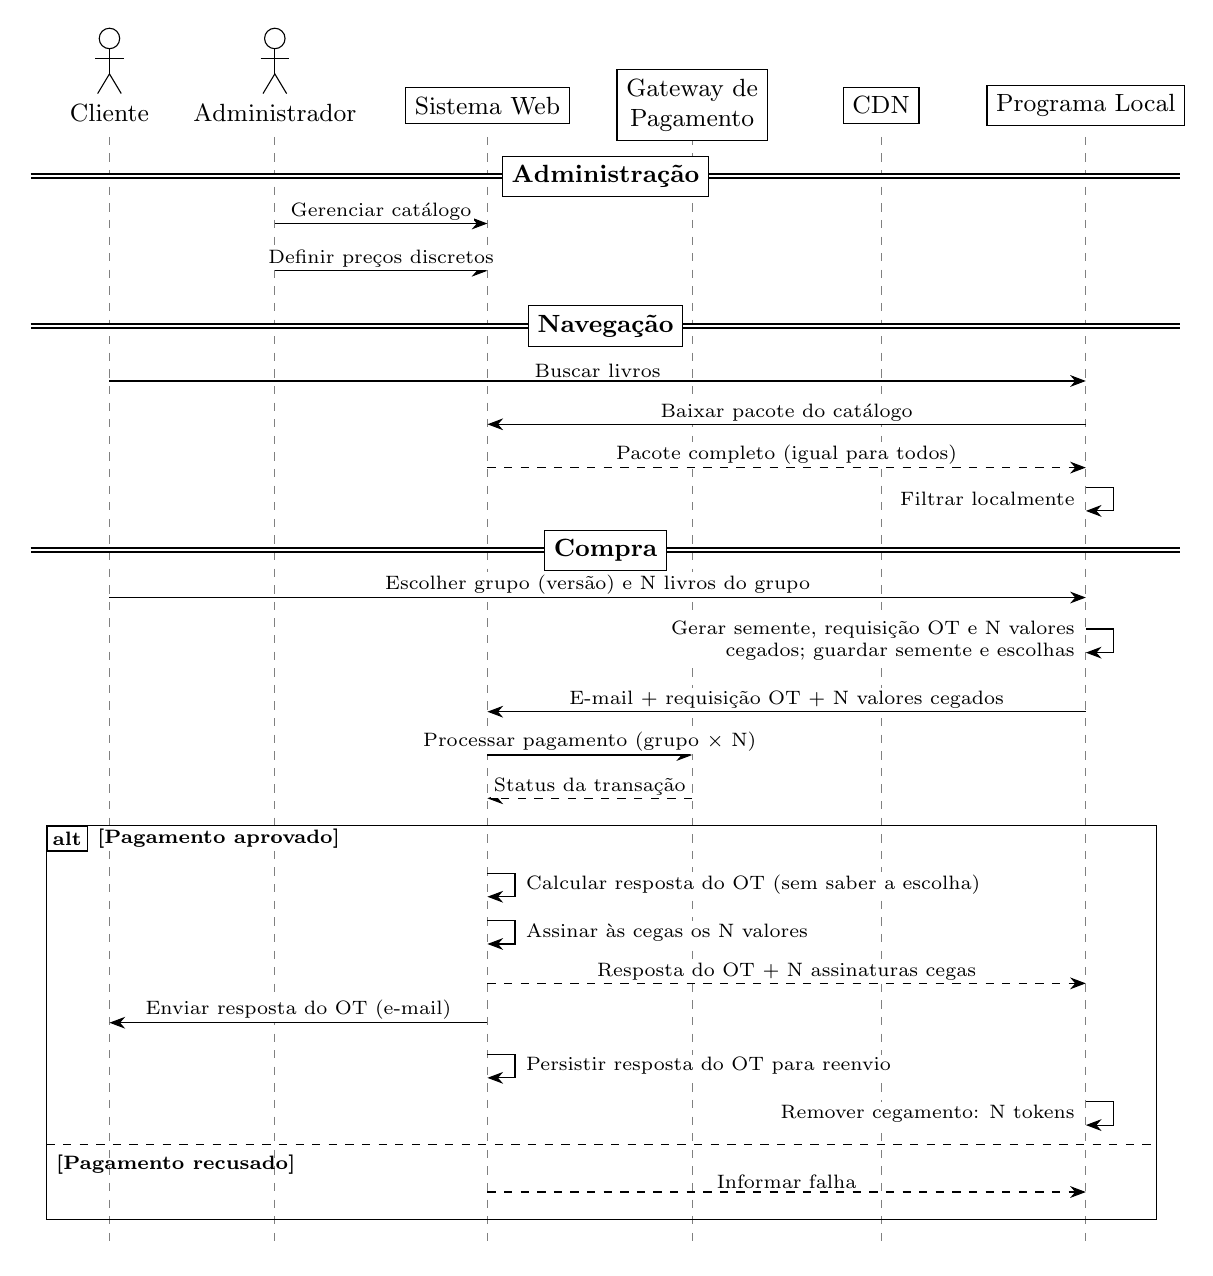
\begin{tikzpicture}
  \sdlifelines{-14.6}
  \sdheads

  \sdbanner{-1.0}{Administração}
  \sdcall{\xAdm}{\xWeb}{-1.6}{Gerenciar catálogo}
  \sdcall{\xAdm}{\xWeb}{-2.2}{Definir preços discretos}

  \sdbanner{-2.9}{Navegação}
  \sdcall{\xCli}{\xPrg}{-3.6}{Buscar livros}
  \sdcall{\xPrg}{\xWeb}{-4.15}{Baixar pacote do catálogo}
  \sdreply{\xWeb}{\xPrg}{-4.7}{Pacote completo (igual para todos)}
  \sdselfL{\xPrg}{-4.95}{Filtrar localmente}

  \sdbanner{-5.75}{Compra}
  \sdcall{\xCli}{\xPrg}{-6.35}{Escolher grupo (versão) e N livros do grupo}
  \sdselfL{\xPrg}{-6.75}{Gerar semente, requisição OT e N valores\\cegados; guardar semente e escolhas}
  \sdcall{\xPrg}{\xWeb}{-7.8}{E-mail + requisição OT + N valores cegados}
  \sdcall{\xWeb}{\xGat}{-8.35}{Processar pagamento (grupo $\times$ N)}
  \sdreply{\xGat}{\xWeb}{-8.9}{Status da transação}

  \sdframe{-0.8}{-9.25}{13.3}{-14.25}{alt}{Pagamento aprovado}
  \sdselfR{\xWeb}{-9.85}{Calcular resposta do OT (sem saber a escolha)}
  \sdselfR{\xWeb}{-10.45}{Assinar às cegas os N valores}
  \sdreply{\xWeb}{\xPrg}{-11.25}{Resposta do OT + N assinaturas cegas}
  \sdcall{\xWeb}{\xCli}{-11.75}{Enviar resposta do OT (e-mail)}
  \sdselfR{\xWeb}{-12.15}{Persistir resposta do OT para reenvio}
  \sdselfL{\xPrg}{-12.75}{Remover cegamento: N tokens}
  \sdelse{-0.8}{13.3}{-13.3}{Pagamento recusado}
  \sdreply{\xWeb}{\xPrg}{-13.9}{Informar falha}
\end{tikzpicture}
\fonte{Elaborado pelos autores.}
\end{figure}

% ---------------------------------------------------------------------------
\begin{figure}[htbp]
\centering
\caption{Diagrama de sequência: entrega, reporte da CDN e descriptografia local}\label{fig:seq-entrega}
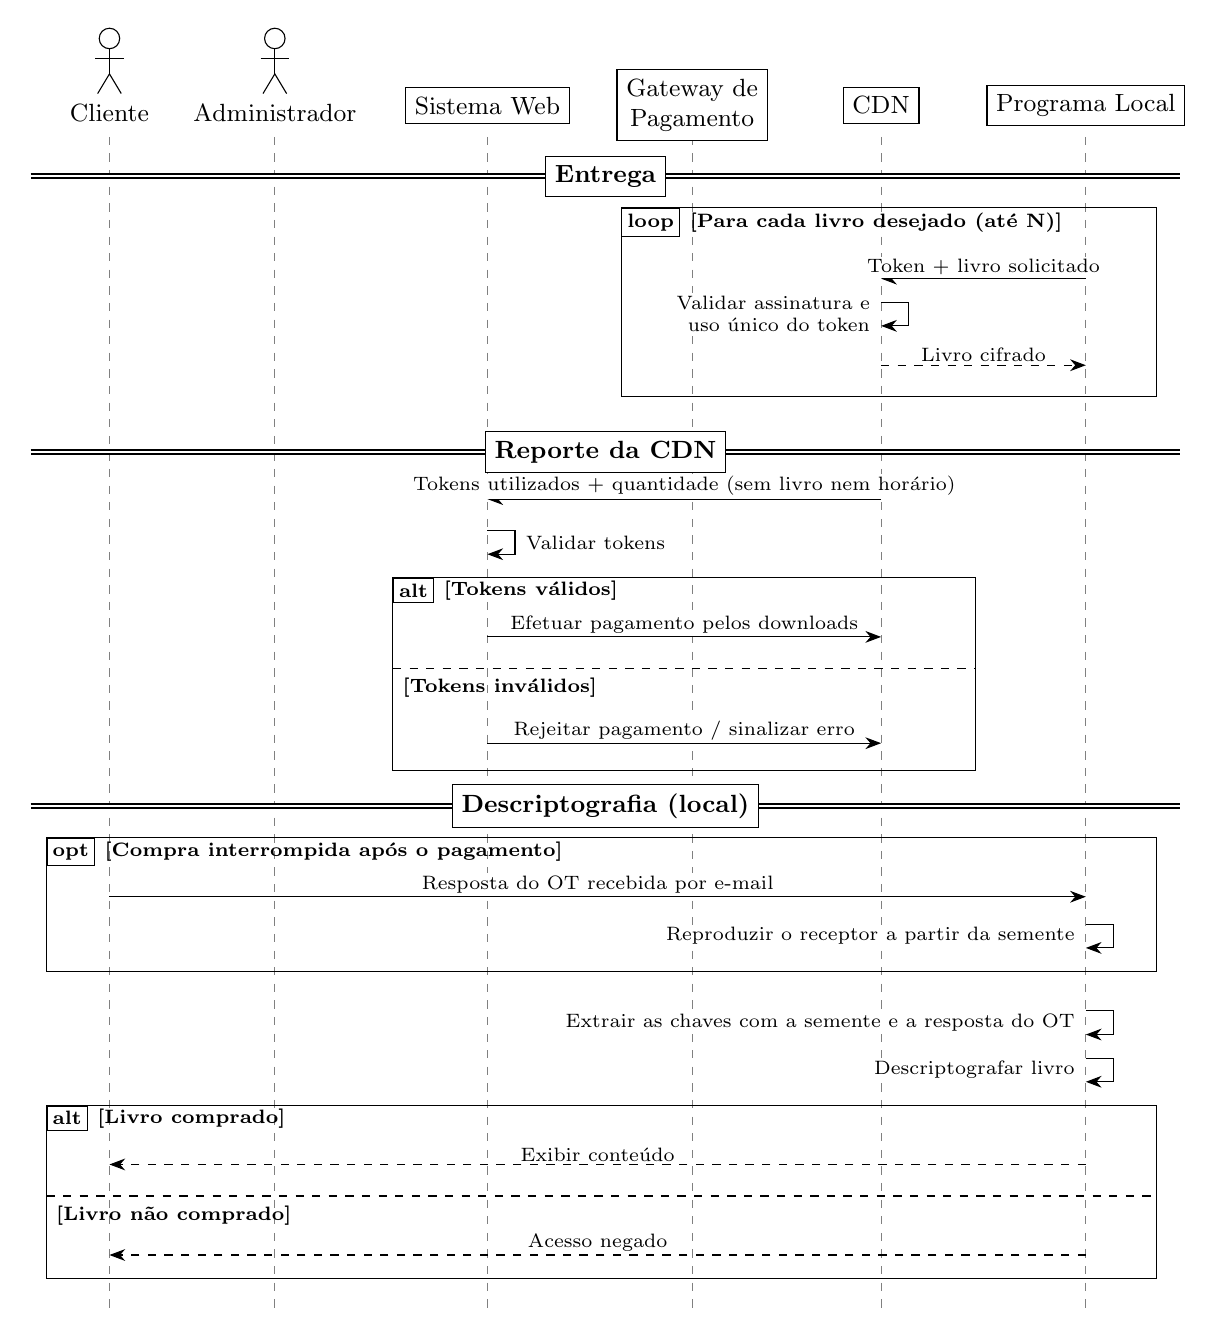
\begin{tikzpicture}
  \sdlifelines{-15.4}
  \sdheads

  \sdbanner{-1.0}{Entrega}
  \sdframe{6.5}{-1.4}{13.3}{-3.8}{loop}{Para cada livro desejado (até N)}
  \sdcall{\xPrg}{\xCdn}{-2.3}{Token + livro solicitado}
  \sdselfL{\xCdn}{-2.6}{Validar assinatura e\\uso único do token}
  \sdreply{\xCdn}{\xPrg}{-3.4}{Livro cifrado}

  \sdbanner{-4.5}{Reporte da CDN}
  \sdcall{\xCdn}{\xWeb}{-5.1}{Tokens utilizados + quantidade (sem livro nem horário)}
  \sdselfR{\xWeb}{-5.5}{Validar tokens}
  \sdframe{3.6}{-6.1}{11.0}{-8.55}{alt}{Tokens válidos}
  \sdcall{\xWeb}{\xCdn}{-6.85}{Efetuar pagamento pelos downloads}
  \sdelse{3.6}{11.0}{-7.25}{Tokens inválidos}
  \sdcall{\xWeb}{\xCdn}{-8.2}{Rejeitar pagamento / sinalizar erro}

  \sdbanner{-9.0}{Descriptografia (local)}
  \sdframe{-0.8}{-9.4}{13.3}{-11.1}{opt}{Compra interrompida após o pagamento}
  \sdcall{\xCli}{\xPrg}{-10.15}{Resposta do OT recebida por e-mail}
  \sdselfL{\xPrg}{-10.5}{Reproduzir o receptor a partir da semente}
  \sdselfL{\xPrg}{-11.6}{Extrair as chaves com a semente e a resposta do OT}
  \sdselfL{\xPrg}{-12.2}{Descriptografar livro}
  \sdframe{-0.8}{-12.8}{13.3}{-15.0}{alt}{Livro comprado}
  \sdreply{\xPrg}{\xCli}{-13.55}{Exibir conteúdo}
  \sdelse{-0.8}{13.3}{-13.95}{Livro não comprado}
  \sdreply{\xPrg}{\xCli}{-14.7}{Acesso negado}
\end{tikzpicture}
\fonte{Elaborado pelos autores.}
\end{figure}


% Capítulo 5. Desenvolvimento do Trabalho
% ===========================================================================
\chapter{Desenvolvimento do Trabalho}\label{cap:desenvolvimento}
% ===========================================================================

Este capítulo apresenta a transformação dos requisitos do
\autoref{cap:especificacao} no produto: as tecnologias utilizadas, o projeto e
a implementação da solução, com as decisões tomadas e as alternativas
descartadas, e os testes e a avaliação. As fases 4 e 5 do método ainda estão
em andamento, e o capítulo registra o estado em que se encontram.

\section{Tecnologias Utilizadas}\label{sec:tecnologias}

Esta seção compara, para cada decisão de projeto, a alternativa escolhida com
as descartadas, usando os mesmos critérios para todas. A comparação é
qualitativa: registra propriedades verificadas no código-fonte ou na
documentação de cada alternativa e marca como ``não verificado'' o que não foi
confirmado.

\subsection{Biblioteca de OT}

Critérios:
(C1) compatibilidade com o fluxo de compra, em que o programa local envia a
requisição e o sistema web responde em uma única mensagem;
(C2) possibilidade de guardar ou reproduzir o estado do receptor entre a
requisição e a extração das chaves (RF11, RF14);
(C3) execução no Windows, ambiente do programa local;
(C4) maturidade e recomendação de uso pelos autores;
(C5) aderência ao foco do trabalho, que é o uso de protocolos de OT.

\begin{table}[H]
\centering
\caption{Comparativo das bibliotecas de OT avaliadas}\label{tab:comp-libs}
\footnotesize
\renewcommand{\arraystretch}{1.25}
\begin{tabularx}{\textwidth}{@{}>{\raggedright\arraybackslash}p{0.13\textwidth}
  >{\raggedright\arraybackslash}X >{\raggedright\arraybackslash}X
  >{\raggedright\arraybackslash}p{0.11\textwidth} >{\raggedright\arraybackslash}X
  >{\raggedright\arraybackslash}p{0.11\textwidth}@{}}
\toprule
\textbf{Alternativa} & \textbf{C1 -- Mensagens} & \textbf{C2 -- Estado do receptor} &
\textbf{C3 -- Windows} & \textbf{C4 -- Maturidade} & \textbf{Resultado} \\
\midrule
libOTe, OT base de \citeonline{masnyrindal2019} &
Compatível: a requisição do receptor não depende da mensagem do \emph{sender},
que segue na resposta &
Em memória, mas reproduzível: toda a aleatoriedade do receptor vem do gerador
recebido como parâmetro (verificado no código) &
Sim, segundo os autores &
Acadêmica, licença MIT, amplamente citada &
\textbf{Escolhida} \\
\addlinespace
emp-ot, protocolo PVW &
Compatível: receptor envia primeiro, duas mensagens &
Em memória, chamada bloqueante; reprodutibilidade não verificada &
\textbf{Não} (apenas Linux e macOS) &
Software de pesquisa, sem auditoria independente, segundo os autores &
Descartada (C3) \\
\addlinespace
circl, Simplest OT &
Exige uma troca adicional: a requisição do receptor depende da mensagem inicial
do \emph{sender} &
API dividida em rodadas, favorável &
Sim &
Apenas 1-out-of-2; pacote fora da versão mais recente do módulo &
Descartada (C1, C4) \\
\addlinespace
mpz, Chou--Orlandi &
Mesma dependência da mensagem inicial do \emph{sender} (protocolo Chou--Orlandi) &
Favorável: máquinas de estado sem rede, com mensagens explícitas &
Não verificado &
Autores recomendam não usar em produção; mudanças incompatíveis frequentes &
Descartada (C4) \\
\addlinespace
swanky (Naor--Pinkas, Chou--Orlandi) &
Não verificado &
Não verificado &
Não verificado &
Autores recomendam não usar em produção &
Descartada (C4) \\
\addlinespace
OPRF (RFC 9497) usado para construir 1-out-of-n &
Compatível: cliente envia primeiro, duas mensagens &
API em passos, favorável &
Sim &
Padronizado, várias implementações independentes &
Descartada (C5) \\
\bottomrule
\end{tabularx}
\fonte{Elaborado pelos autores a partir da documentação e do código-fonte das bibliotecas.}
\end{table}

A alternativa baseada em função pseudoaleatória oblívia (\emph{Oblivious Pseudorandom Function} -- OPRF), padronizada no documento RFC (\emph{Request for Comments}) 9497, é tecnicamente adequada, mas não é um protocolo
de OT: ela obtém a funcionalidade de 1-out-of-n a partir de uma função
pseudoaleatória avaliada obliviamente, o que deslocaria o foco do trabalho.


\subsection{Tecnologias do sistema web}

\begin{table}[H]
\centering
\caption{Comparativo das tecnologias do sistema web}\label{tab:comp-stack}
\footnotesize
\renewcommand{\arraystretch}{1.25}
\begin{tabularx}{\textwidth}{@{}>{\raggedright\arraybackslash}p{0.14\textwidth}
  >{\raggedright\arraybackslash}p{0.2\textwidth} >{\raggedright\arraybackslash}p{0.2\textwidth}
  >{\raggedright\arraybackslash}X@{}}
\toprule
\textbf{Tema} & \textbf{Escolhida} & \textbf{Descartada} & \textbf{Motivo} \\
\midrule
Linguagem & Go & TypeScript (Node.js); Python &
Go oferece assinatura cega RSA padronizada \cite{rfc9474} em biblioteca
mantida, biblioteca padrão com servidor HTTP (\emph{Hypertext Transfer Protocol}) e criptografia, e binário único.
Em Python não foi identificada implementação consolidada da RFC 9474. \\
\addlinespace
Banco de dados & PostgreSQL & SQLite &
Escritas concorrentes representativas para o teste de carga (RNF05). \\
\addlinespace
Interface & HTML (\emph{HyperText Markup Language}) gerado no servidor & Aplicação de página única (SPA) &
Menor superfície de ataque e nenhuma dependência de código de terceiros no
navegador. \\
\addlinespace
Busca (RF04) & Pacote completo, navegado no programa local & Vitrine no
navegador com filtro local; busca no servidor sem registros &
Na vitrine no navegador, o filtro é código fornecido pelo sistema web, e a
proteção dependeria de ele ser honesto; na busca no servidor, o sistema web
observa as consultas e a proteção dependeria apenas de disciplina
operacional. \\
\addlinespace
Acesso à biblioteca de OT & Binário auxiliar & Ligação direta ao código C++ &
Isola o código C++ e desacopla a compilação da biblioteca da compilação do
sistema web. \\
\bottomrule
\end{tabularx}
\fonte{Elaborado pelos autores.}
\end{table}


\section{Projeto e Implementação}\label{sec:projeto}

\subsection{Visão geral da solução}

A partir dos requisitos, a ideia inicial do projeto é uma plataforma de venda
de chaves de livros criptografados, que são distribuídos por uma CDN. A
solução é composta por três componentes:

\begin{enumerate}
\item \textbf{Sistema web (site):} administração e publicação do catálogo,
preços discretos, pagamento via gateway, execução do OT e assinatura cega de
tokens. A compra não exige conta; apenas o e-mail é solicitado.

\item \textbf{CDN:} armazena os livros cifrados e entrega um livro mediante um
token com assinatura cega válido. Posteriormente, reporta ao site os tokens
utilizados para ser remunerada.

\item \textbf{Programa local:} instalado no computador do cliente, baixa o
catálogo completo e permite buscar e navegar localmente, gera a requisição de
OT e guarda seu segredo, comunica-se com o sistema web e com a CDN, remove o
cegamento dos tokens e descriptografa os livros localmente.
\end{enumerate}

No fluxo de compra, o cliente escolhe um grupo de livros de mesmo preço e
obtém, por meio do OT, as chaves de N itens desse grupo, sem que o site saiba
quais foram escolhidos. O cliente recebe também N tokens com assinatura cega,
com os quais baixa os livros cifrados na CDN, e em seguida os descriptografa
localmente. Como cada download consome um token e a CDN reporta os tokens
utilizados, torna-se possível a remuneração justa da CDN sem revelar ao site
quais livros foram adquiridos.

A execução do OT é síncrona: durante a compra, o programa local envia a
requisição de OT e recebe a resposta em uma única troca de mensagens com o
sistema web, dentro do limite de RNF03. Toda a aleatoriedade do lado receptor
é derivada de uma semente guardada pelo programa local (RF11); por isso, se a
compra for interrompida após o pagamento, o programa reproduz o estado do
receptor a partir da semente e extrai as chaves usando a resposta do OT
recebida por e-mail (RF14). Esse desenho exige um protocolo de OT em que o
sistema web responda em uma única mensagem e em que o estado do receptor seja
reproduzível a partir da semente.

Os livros de um grupo de mesmo preço são organizados em versões imutáveis: a
inclusão, remoção ou alteração de preço de um livro gera uma nova versão do
grupo, e cada compra referencia a versão sobre a qual os índices do OT foram
escolhidos.


\subsection{Decisões de projeto}

\begin{itemize}
\item \textbf{Execução do OT:} síncrona na compra, com o estado do receptor
reproduzível a partir de uma semente guardada pelo programa local (RF11,
RF14).

\item \textbf{Biblioteca de OT:} libOTe \cite{libote}, com o protocolo de
\citeonline{masnyrindal2019} como OT base 1-out-of-2. A compilação no ambiente
do cliente e a reprodutibilidade do receptor a partir da semente são
verificadas por testes automatizados durante a implementação.

\item \textbf{Sistema web:} linguagem Go, banco PostgreSQL, páginas de
administração renderizadas no servidor, sem recursos de terceiros; catálogo
publicado como pacote completo, sem vitrine pública; biblioteca de OT acessada
por um binário auxiliar. A única página pública é a de apresentação e
download, sem cookies, scripts ou recursos de terceiros, que exibe a versão,
o resumo SHA-256 (\emph{Secure Hash Algorithm}) e a chave pública do catálogo atual para que qualquer pessoa
possa conferi-los.

\item \textbf{Navegação e busca:} no programa local, sobre o pacote completo
do catálogo. As capas seguem no pacote como miniaturas de 200 por 300 pixels em
JPEG (\emph{Joint Photographic Experts Group}), geradas no envio da capa, para que o tamanho do pacote não dependa das
imagens originais.

\item \textbf{Pacote do catálogo:} um arquivo ZIP único por versão, com os
metadados em JSON (\emph{JavaScript Object Notation}) e as miniaturas. O arquivo é gerado de forma
determinística, de modo que o mesmo conteúdo produz sempre os mesmos bytes e o
resumo SHA-256 identifica a versão. O programa local sempre baixa o pacote
completo, revalidando-o pelo resumo, para que todos os clientes façam a mesma
requisição. O sistema web assina cada versão com Ed25519 e publica versão,
resumo e assinatura, o que permite a qualquer pessoa verificar que recebeu o
mesmo catálogo que os demais. O programa local confere a assinatura com a
chave pública embutida e recusa versões anteriores à que já possui.

\item \textbf{Assinatura cega:} RSA cego padronizado \cite{rfc9474}, com
módulo de 3072 bits (RNF01) e uma chave por faixa de preço. A chave pública de
cada faixa vai no pacote assinado do catálogo, de modo que todos os clientes e
a CDN recebem a mesma chave e o sistema web não consegue reconhecer os tokens
de um cliente específico.

\item \textbf{Variante de OT:} o OT 1-out-of-n de \citeonline{naorpinkas1999},
repetido N vezes. Cada execução usa $\lceil \log_2 n \rceil$ OTs 1-out-of-2 do
MR19. A chave do livro de índice $i$ é cifrada com um resumo SHA-256 das chaves
dos OTs correspondentes aos bits de $i$. A privacidade da escolha diante do
sistema web é garantia do protocolo; a de que o cliente não abre outras
posições depende de modelar o SHA-256 como oráculo aleatório (premissa).

\item \textbf{Cifra dos livros:} AES-256-GCM, com uma chave aleatória por livro
e o identificador do livro como dado associado.

\item \textbf{Grupos, reenvio e pagamento:} grupo mínimo de 5 livros; reenvio
da resposta do OT por 30 dias; gateway de pagamento simulado atrás de uma
interface, cobrando o preço da faixa vezes N.

\item \textbf{Tokens e reporte:} cada token vale um único download. A CDN
reporta em lotes de 50 tokens ou uma vez por dia, embaralhados, sem horários e
sem livro.

\item \textbf{Semente:} toda a aleatoriedade do cliente numa compra (receptor
do OT, mensagens dos tokens e fatores de cegamento) é derivada de uma semente
de 256 bits gravada antes do envio. Com ela e a resposta recebida por e-mail, o
programa local refaz a compra interrompida.

\item \textbf{Programa local:} em Go, com linha de comando e uma janela gráfica
para Windows que usa o componente WebView2. A página da janela é embutida no
executável e não acessa a rede: todas as operações passam pelo código do
programa, que se conecta apenas ao sistema web e à CDN.

\item \textbf{Remuneração da CDN:} tarifa fixa por token entregue; o sistema
web registra a quantidade e o valor de cada lote.

\item \textbf{Falha seletiva no OT:} o programa local troca todos os tokens na
CDN antes de decifrar e não informa ao sistema web se alguma chave falhou, de
modo que sua comunicação é a mesma em qualquer caso.

\item \textbf{Interface:} um único tema visual para os três componentes, com
fontes servidas pelos próprios componentes, sem recursos de terceiros.
\end{itemize}


\subsection{Alternativas de projeto descartadas}\label{sec:alternativas}

As alternativas a seguir são comparadas com o mesmo método da
\autoref{sec:tecnologias}.

\subsubsection{Execução do OT}

Critérios: utilidade do envio da resposta por e-mail (RF14) e do reenvio
(RF15); recuperação de uma compra interrompida após o pagamento (RNF07);
quantidade de código criptográfico próprio.

\begin{table}[H]
\centering
\caption{Comparativo das formas de execução do OT}\label{tab:comp-execucao}
\footnotesize
\renewcommand{\arraystretch}{1.25}
\begin{tabularx}{\textwidth}{@{}>{\raggedright\arraybackslash}p{0.2\textwidth}
  >{\raggedright\arraybackslash}X >{\raggedright\arraybackslash}X
  >{\raggedright\arraybackslash}X >{\raggedright\arraybackslash}p{0.12\textwidth}@{}}
\toprule
\textbf{Alternativa} & \textbf{RF14 e RF15} & \textbf{Compra interrompida} &
\textbf{Código criptográfico próprio} & \textbf{Resultado} \\
\midrule
Síncrona, com semente guardada &
Úteis: a resposta recebida por e-mail permite extrair as chaves &
Recuperável a partir da semente &
Nenhum além de inicializar o gerador com a semente; depende da premissa de
determinismo do receptor &
\textbf{Escolhida} \\
\addlinespace
Síncrona, sem estado guardado &
Perdem a utilidade: sem o segredo, a resposta não serve &
Irrecuperável: o cliente paga e perde a compra &
Nenhum &
Descartada \\
\addlinespace
Adaptador com estado serializado &
Úteis &
Recuperável a partir do estado salvo &
Reorganização do protocolo em duas etapas sobre as primitivas da biblioteca &
Descartada \\
\bottomrule
\end{tabularx}
\fonte{Elaborado pelos autores.}
\end{table}


\subsubsection{Onde executa o receptor do OT}

Critérios: natureza da privacidade da escolha (RF07), usabilidade, viabilidade
técnica com a biblioteca escolhida e armazenamento da semente (RF11).

\begin{table}[H]
\centering
\caption{Comparativo dos locais de execução do receptor}\label{tab:comp-receptor}
\footnotesize
\renewcommand{\arraystretch}{1.25}
\begin{tabularx}{\textwidth}{@{}>{\raggedright\arraybackslash}p{0.19\textwidth}
  >{\raggedright\arraybackslash}X >{\raggedright\arraybackslash}X
  >{\raggedright\arraybackslash}X >{\raggedright\arraybackslash}X
  >{\raggedright\arraybackslash}p{0.11\textwidth}@{}}
\toprule
\textbf{Alternativa} & \textbf{Privacidade da escolha} & \textbf{Usabilidade} &
\textbf{Biblioteca de OT} & \textbf{Semente} & \textbf{Resultado} \\
\midrule
Programa local com acesso restrito ao sistema web e à CDN &
Garantia do protocolo &
Sem transporte manual de arquivos &
Execução nativa &
Disco do cliente &
\textbf{Escolhida} \\
\addlinespace
Programa local sem rede (versão 2 desta especificação) &
Garantia do protocolo &
Cliente transporta arquivos entre navegador e programa &
Execução nativa &
Disco do cliente &
Descartada \\
\addlinespace
Navegador, com código fornecido pelo sistema web &
Premissa: o servidor fornece código honesto &
Nada a instalar &
Exigiria compilação para WebAssembly (viabilidade não verificada) &
Guardada no navegador, sujeita a remoção &
Descartada \\
\addlinespace
Navegador, com código de outra origem (extensão ou página estática auditável) &
Premissa mais fraca: código auditável e independente do servidor &
Instalação de extensão ou uso de página separada &
Mesma limitação da alternativa anterior &
Guardada no navegador &
Descartada \\
\bottomrule
\end{tabularx}
\fonte{Elaborado pelos autores.}
\end{table}


\subsection{Estado da implementação}\label{sec:estado}

Esta seção registra o andamento da Fase 4 em 22 de novembro de 2026. Os
três componentes estão implementados e o fluxo de compra roda de ponta a
ponta. O código está no
repositório do projeto (\url{https://github.com/migs39/tcc}).

\begin{table}[H]
\centering
\caption{Passos da implementação do sistema web}\label{tab:passos}
\footnotesize
\renewcommand{\arraystretch}{1.2}
\begin{tabularx}{\textwidth}{@{}>{\raggedright\arraybackslash}p{0.075\textwidth}
  >{\raggedright\arraybackslash}X >{\raggedright\arraybackslash}p{0.22\textwidth}
  >{\raggedright\arraybackslash}p{0.15\textwidth}@{}}
\toprule
\textbf{Passo} & \textbf{Entrega} & \textbf{Requisitos} & \textbf{Situação} \\
\midrule
0 & Base: banco de dados, migrações e testes isolados & --- & Concluído \\
1 & Cadastro, autenticação e gestão de administradores & RF01, UC01 & Concluído \\
2 & Catálogo, preços discretos, capas e grupos versionados & RF02, RF03, RF07, UC02, UC03 & Concluído \\
3 & Pacote do catálogo e página pública & RF04, UC04 & Concluído \\
4 & Compra sem conta, e-mail e pagamento & RF05, RF06, RF13 & Concluído \\
5 & Envio da resposta do OT por e-mail & RF14, RNF04 & Concluído \\
6 & OT no sistema web, com a biblioteca libOTe & RF07, RF08 & Concluído \\
7 & Emissão de tokens com assinatura cega & RF16 & Concluído \\
8 & Recebimento e validação do reporte da CDN & RF18, UC17 & Concluído \\
9 & Reenvio da resposta do OT & RF15 & Concluído \\
10 & Testes de privacidade e de carga & RNF02--RNF05 & Parcial \\
\bottomrule
\end{tabularx}
\fonte{Elaborado pelos autores.}
\end{table}


\subsubsection{O que os passos concluídos entregam}

\begin{itemize}
\item \textbf{Administradores (RF01):} cadastro, autenticação e gestão de
perfis, inclusive desativação, que nunca deixa o sistema sem administrador
ativo. As senhas são guardadas com argon2id; a sessão usa um token aleatório
de 256 bits, do qual só o resumo fica no banco. Requisições de alteração
vindas de outra origem são recusadas.

\item \textbf{Catálogo e preços (RF02, RF03):} livros com título, autor,
categoria, descrição, ano, ISBN (\emph{International Standard Book Number}), editora e capa; faixas de preço e categorias
mantidas pelo administrador. A restrição de preço ao conjunto pré-definido é
imposta pelo código e também pelo banco de dados, de modo que nenhum livro
fica com preço fora do conjunto mesmo que o código seja contornado. Remover
um livro o desativa, preservando as versões de grupo que o referenciam.

\item \textbf{Grupos versionados (RF07):} cada mudança na composição de um
grupo de mesmo preço gera uma versão imutável; editar dados de um livro sem
mudar seu preço não gera versão. A posição do livro na versão é o índice
usado pelo OT.

\item \textbf{Pacote do catálogo (RF04):} o sistema web publica o catálogo
como um arquivo ZIP determinístico, com os metadados dos livros ativos, as
versões atuais dos grupos e as miniaturas das capas, assinado com Ed25519. A
página pública de apresentação e download mostra a versão, o resumo e a chave
pública do catálogo atual.
\end{itemize}


\subsubsection{Compra, CDN e programa local}

\begin{itemize}
\item \textbf{Compra (RF05--RF08, RF13, RF16):} o programa local envia o
e-mail, a versão do grupo, N, a requisição do OT e os N valores cegados. O
sistema web roda o lado \emph{sender} do OT, cobra o grupo vezes N, assina os
valores às cegas e devolve a resposta do OT com as assinaturas. Uma
requisição inválida é recusada antes da cobrança.
\item \textbf{E-mail e reenvio (RF14, RF15):} a resposta do OT vai por e-mail,
fora da requisição, e pode ser reenviada ao e-mail original por 30 dias. Ela
não contém chave alguma.
\item \textbf{CDN (RF17, RF18):} guarda os livros cifrados, entrega um livro
por token válido da faixa do livro e ainda não usado e reporta os tokens em
lotes. O sistema web confere cada assinatura e recusa tokens repetidos.
\item \textbf{Programa local (RF04, RF10--RF12):} baixa e confere o catálogo,
faz a busca localmente, grava a semente antes do envio, compra, troca os tokens
por livros na CDN, extrai as chaves e decifra no computador do cliente.
\end{itemize}

O binário auxiliar que expõe o libOTe compila no Windows e no Linux, e a
requisição do receptor é idêntica byte a byte quando gerada com a mesma
semente, o que confirma a premissa da execução síncrona com semente.

\subsection{Questões em aberto}

\begin{itemize}
\item Valor da remuneração da CDN por token (o sistema web já registra a
quantidade por lote).
\item Proteção da semente armazenada no programa local, além da permissão do
arquivo.
\item Compromissos das chaves dos livros no pacote do catálogo, para o
programa local conferir as chaves extraídas (defesa contra o ataque de falha
seletiva no OT).
\item Interface gráfica do programa local.
\item Integração com um gateway de pagamento e um serviço de e-mail reais.
\item Momento do download logo após a compra, que a CDN observa; o programa
local permite adiar o download.
\end{itemize}

% ---------------------------------------------------------------------------

\section{Testes e Avaliação}\label{sec:testes}

\subsection{Testes automatizados}

O sistema web tem 29 testes automatizados, executados contra um banco
PostgreSQL real, cada teste em um esquema isolado. Os grupos de testes são:

\begin{itemize}
\item \textbf{Administradores (9 testes):} formato e verificação do resumo de
senha; cadastro e validações; autenticação; desativação, que encerra sessões
e bloqueia o acesso; troca de senha, que encerra as sessões; sessão guardada
apenas como resumo.
\item \textbf{Catálogo (9 testes):} preço fora do conjunto recusado pelo
código e pelo banco (RF03); regras de faixas e categorias; validação de ano e
ISBN; sequência e imutabilidade das versões de grupo; capas e miniaturas.
\item \textbf{Pacote do catálogo (3 testes):} conteúdo e ordem dos grupos;
determinismo; geração de versões; recusa de pacote adulterado, de número de
versão trocado e de chave errada.
\item \textbf{Interface web (8 testes):} acesso administrativo restrito a
administradores autenticados; recusa de requisições de outra origem; fluxo
completo do catálogo; revalidação do pacote; página pública sem cookies,
scripts ou recursos de terceiros.
\end{itemize}

Os demais componentes acrescentam os seguintes grupos de testes:

\begin{itemize}
\item \textbf{Protocolo (6 testes):} o cliente recupera exatamente as chaves
escolhidas e nenhuma outra posição abre (RF12); a mesma semente gera a mesma
requisição; o tamanho da requisição não depende da escolha; tokens válidos,
reproduzíveis a partir da semente e diferentes do que o sistema web viu
(RF16); cifra dos livros.
\item \textbf{Compra (7 testes):} compra de ponta a ponta com o binário do
libOTe; registros e respostas de mesma forma e tamanho para escolhas
diferentes; e-mail sem chave; cobrança pelo grupo vezes N; pagamento recusado
sem registro; validações; reenvio dentro e fora do prazo; reporte da CDN
válido, repetido e adulterado.
\item \textbf{CDN (1 teste):} entrega só com token da faixa do livro, uma única
vez; reporte em lote; tabela de tokens sem livro nem horário.
\end{itemize}

Um teste de ponta a ponta com os três componentes cobriu o cadastro de livros,
o envio dos arquivos à CDN, a compra de dois livros de um grupo de seis, a
decifragem, as recusas (grupo pequeno, grupos diferentes, pagamento recusado),
a recuperação de uma compra pelo e-mail e o reporte da CDN aceito pelo sistema
web. Falta o teste de carga concorrente para RNF05.


\subsection{Medições}

As miniaturas de capa, de 200 por 300 pixels em JPEG, mediram de 1,6~KB (capa
de cor lisa) a 19,8~KB (pior caso, imagem de ruído aleatório). Com mil livros,
o pacote do catálogo fica abaixo de cerca de 20~MB.

Com um grupo de 100 livros e N = 5, uma compra leva cerca de 58~ms no sistema
web, num computador de dois núcleos. O tempo inclui o \emph{sender} do OT, as
cifras de Naor--Pinkas, a cobrança simulada, cinco assinaturas RSA de 3072
bits e a gravação. Isso dá cerca de mil compras por minuto em um núcleo, acima
das 600 de RNF05, e fica muito abaixo do limite de um minuto de RNF03. A
requisição do OT tem 1.256 bytes para 19 OTs e a resposta do \emph{sender},
64 bytes.


% ---
% Capitulo com exemplos de comandos inseridos de arquivo externo 
% ---
% \include{abntex2-modelo-include-comandos}
% ---
% Conteúdos específicos do modelo de trabalho acadêmico
% \include{quadros}

% ----------------------------------------------------------
% Finaliza a parte no bookmark do PDF
% para que se inicie o bookmark na raiz
% e adiciona espaço de parte no Sumário
% ----------------------------------------------------------
\phantompart

% ---
% Conclusão
% ---
% Capítulo 6. Considerações Finais
% Entra quando o app estiver concluído e testado:
% % ===========================================================================
\chapter{Considerações Finais}\label{cap:consideracoes}
% ===========================================================================

Este capítulo faz o balanço do trabalho em relação aos objetivos do
\autoref{cap:introducao}, aponta o que é contribuição dos autores e indica
caminhos para continuar o projeto.

\section{Conclusões do Projeto de Formatura}

O objetivo geral foi atingido. O protótipo vende livros digitais organizados em
grupos de mesmo preço, entrega ao cliente as chaves dos N livros escolhidos por
meio de \emph{Oblivious Transfer} e distribui os livros cifrados por uma CDN,
de modo que a loja recebe o pagamento sem saber quais livros foram comprados.
O fluxo roda de ponta a ponta com os três componentes previstos, e todos os
requisitos funcionais essenciais foram implementados e verificados pela
bateria controlada da \autoref{sec:testes}.

Quanto aos objetivos específicos:

\begin{itemize}
\item \textbf{Arquitetura:} a separação entre sistema web, CDN e programa local
foi mantida do início ao fim. A principal revisão foi permitir que o programa
local acesse a rede, restrito ao sistema web e à CDN, o que eliminou o
transporte manual de arquivos sem enfraquecer a garantia sobre a escolha,
porque o código do receptor continua fora do controle do sistema web.

\item \textbf{Algoritmo criptográfico:} o OT 1-out-of-n de
\citeonline{naorpinkas1999}, repetido N vezes sobre o OT base de
\citeonline{masnyrindal2019}, foi integrado por meio da biblioteca libOTe. O
custo, de N vezes $\lceil \log_2 n \rceil$ OTs base por compra, mostrou-se
pequeno o bastante para dispensar OT \emph{Extension} nos tamanhos de grupo do
protótipo.

\item \textbf{Legitimidade sem revelar o conteúdo:} a cobrança pelo grupo e
pela quantidade, os tokens de uso único com assinatura cega e o reporte da CDN
apenas com tokens e quantidade permitem cobrar o cliente e remunerar a CDN sem
que o sistema web aprenda os livros comprados.

\item \textbf{Testes de segurança e desempenho:} os testes mostram que o que o
sistema web grava, registra e responde não varia com a escolha, e que nenhuma
chave sai do computador do cliente. As metas de tempo de busca e de compra
foram atendidas com folga, e a de vazão foi atendida a partir de quatro
núcleos.
\end{itemize}

Alguns resultados não foram atingidos ou ficaram parciais. A disponibilidade
(RNF06), a taxa de compras concluídas sem suporte (RNF07) e o tempo de
manutenção (RNF08) dependem de operação real e de estudo com usuários, que
ficaram fora do alcance de um protótipo. O pagamento usa um \emph{gateway}
simulado, porque um real exige conta de lojista, e a janela gráfica existe
apenas para Windows. A defesa contra o ataque de falha seletiva no OT é uma
escolha de engenharia, e não uma garantia formal. Por fim, a não conivência
entre o sistema web e a CDN continua sendo uma premissa: o sistema reduz o que
cada parte aprende, mas não impede que as duas juntem o que sabem.

\section{Contribuições}

A literatura sobre OT com preço e transações oblívias concentra-se nos
protocolos e em suas provas. A contribuição deste trabalho é de engenharia: um
sistema completo, que integra o OT a pagamento, entrega e remuneração, e a
análise do que cada decisão preserva ou enfraquece. São de autoria da equipe:

\begin{itemize}
\item a arquitetura em três componentes com separação de conhecimento entre
sistema web, CDN e \emph{gateway}, e a tabela do que cada parte pode saber,
usada para revisar o código e o esquema do banco;
\item a simplificação do OT com preço por grupos de mesmo preço, cobrando pelo
grupo e pela quantidade, com versões imutáveis dos grupos para fixar os
índices do OT;
\item a recuperação de compras interrompidas a partir de uma semente da qual
deriva toda a aleatoriedade do cliente, inclusive o receptor do OT e o
cegamento dos tokens, o que torna útil o envio da resposta por e-mail sem
alterar a biblioteca de OT nem guardar seu estado interno;
\item a remuneração da CDN por tokens de assinatura cega, com uma chave por
faixa de preço publicada no catálogo assinado, e o reporte em lotes
embaralhados, sem livro nem horário;
\item o catálogo como pacote determinístico, assinado e igual para todos, que
leva a navegação e a busca para o computador do cliente e permite detectar um
catálogo personalizado;
\item a implementação dos três componentes, do binário auxiliar sobre o libOTe,
dos testes de privacidade e da bateria controlada de ponta a ponta.
\end{itemize}

As primitivas criptográficas não são de autoria da equipe e vêm de bibliotecas
consolidadas: o OT base do libOTe, a assinatura cega RSA da biblioteca circl e
as cifras, resumos e assinaturas da biblioteca padrão da linguagem Go. A
construção de Naor e Pinkas sobre os OTs base foi implementada pela equipe a
partir do artigo original.

\section{Perspectivas de Continuidade}

\begin{itemize}
\item \textbf{Compromissos das chaves no catálogo:} publicar no pacote
assinado um compromisso da chave de cada livro, para que o programa local
confira as chaves extraídas e a defesa contra a falha seletiva deixe de
depender apenas do comportamento uniforme.

\item \textbf{Conjunto de anonimato e correlação de horários:} estudar o
tamanho mínimo de grupo e de faixa em função do volume de compras, atrasos ou
lotes no download e o uso de redes de anonimato, para reduzir o que se pode
inferir mesmo com conivência entre o sistema web e a CDN.

\item \textbf{Pagamento real com privacidade:} integrar um \emph{gateway} real
e avaliar meios de pagamento que também escondam a identidade do comprador,
tema que ficou fora do escopo.

\item \textbf{Desempenho:} reduzir o custo das assinaturas cegas, que dominam o
tempo da compra, e avaliar OT \emph{Extension} ou OT k-out-of-n para grupos e
quantidades maiores.

\item \textbf{Portabilidade e usabilidade:} levar a janela gráfica a outros
sistemas operacionais, oferecer cópia de segurança cifrada da semente e
conduzir um estudo com usuários para avaliar RNF07.

\item \textbf{Operação:} implantar o sistema web e a CDN em servidores
independentes, operados por partes diferentes, e medir disponibilidade e vazão
em condições reais.
\end{itemize}


% ----------------------------------------------------------
% ELEMENTOS PÓS-TEXTUAIS
% ----------------------------------------------------------
\postextual
% ----------------------------------------------------------

% ----------------------------------------------------------
% Referências bibliográficas
% ----------------------------------------------------------
\bibliography{referencias}

% ----------------------------------------------------------
% Glossário
% ----------------------------------------------------------
%
% Consulte o manual da classe abntex2 para orientações sobre o glossário.
%
%\glossary

% ----------------------------------------------------------
% Apêndices
% ----------------------------------------------------------

% ---
% Inicia os apêndices
% ---
% \begin{apendicesenv}

% % Imprime uma página indicando o início dos apêndices
% \partapendices

% % ----------------------------------------------------------
% \chapter{Quisque libero justo}
% % ----------------------------------------------------------

% \lipsum[50]

% % ----------------------------------------------------------
% \chapter{Nullam elementum urna vel imperdiet sodales elit ipsum pharetra ligula
% ac pretium ante justo a nulla curabitur tristique arcu eu metus}
% % ----------------------------------------------------------
% \lipsum[55-57]

% \end{apendicesenv}
% % ---


% ----------------------------------------------------------
% Anexos
% ----------------------------------------------------------

% ---
% Inicia os anexos
% ---
% \begin{anexosenv}

% % Imprime uma página indicando o início dos anexos
% \partanexos

% % ---
% \chapter{Morbi ultrices rutrum lorem.}
% % ---
% \lipsum[30]

% % ---
% \chapter{Cras non urna sed feugiat cum sociis natoque penatibus et magnis dis
% parturient montes nascetur ridiculus mus}
% % ---

% \lipsum[31]

% % ---
% \chapter{Fusce facilisis lacinia dui}
% % ---

% \lipsum[32]

% \end{anexosenv}

%---------------------------------------------------------------------
% INDICE REMISSIVO
%---------------------------------------------------------------------
\phantompart
\printindex
%---------------------------------------------------------------------

\end{document}